% Author: Ramón Jaramillo
%\documentclass[tikz,14pt,border=10pt]{standalone}
\documentclass{article}
\usepackage[paperheight=7.75in,paperwidth=5in,margin=0.25in,heightrounded]{geometry}

\usepackage{tikz}
\usepackage{textcomp}
\usetikzlibrary{shapes,arrows}
\begin{document}
% Definition of blocks:
\tikzset{%
  block/.style    = {draw, thick, rectangle, minimum height = 3em,
    minimum width = 3em},
  sum/.style      = {draw, circle, node distance = 2cm}, % Adder
  input/.style    = {coordinate}, % Input
  output/.style   = {coordinate} % Output
}
% Defining string as labels of certain blocks.
\newcommand{\suma}{\Large$+$}
\newcommand{\inte}{$\displaystyle \int$}
\newcommand{\derv}{\huge$\frac{d}{dt}$}



%%%  NULL MODEL


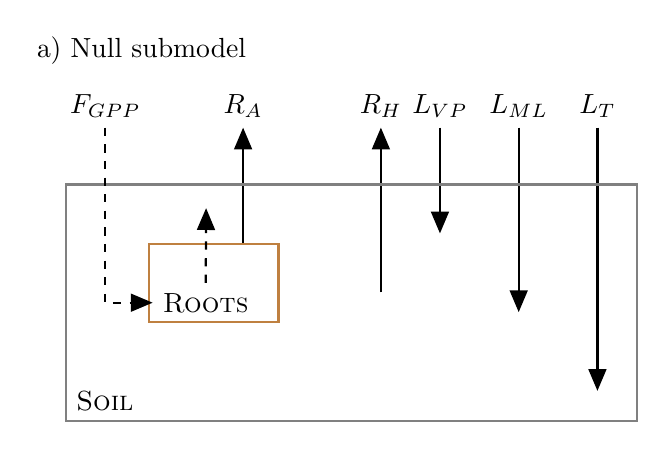
\begin{tikzpicture}[auto, thick, node distance=2cm, >=triangle 45]
%%%

%\node (A) at (2.5, -0.5) {};
%\node (B) at (2.5, 2) {$R_{G}$};

\node (C) at (3.0, -0.5) {};
\node (D) at (3.0, 2) {$R_{H}$};

\node (E) at (1.25, -0.5) {};
\node (F) at (1.25, 2) {$R_{A}$};

\node (G) at (-0.5, 2) {$F_{GPP}$};

\node (Ls) at (3.75, 2) {$L_{VP}$};
\node (Lm) at (4.75, 2) {$L_{ML}$};
\node (Lw) at (5.75, 2) {$L_{T}$};
\node (Ls1) at (3.75, 0.25) {};
\node (Lm1) at (4.75, -0.75) {};
\node (Lw1) at (5.75, -1.75) {};

\node (M) at (3, -0.5) {};
%\node at (0, 2.25) {Microbe \& Microbe-TD};
% arrows
%\draw[->] (A) -- (B);
  \draw[->] (C) -- (D);     
  \draw[->] (E) -- (F);

  \draw[->] (Ls) -- (Ls1);     
  \draw[->] (Lw) -- (Lw1);  
    \draw[->] (Lm) -- (Lm1);  
  
  

\node (C1-root) at (-0.4, 0.5)  {};
  
%\draw [dashed,color=gray,thick] (-1.0,0 )-- (8,0);
%\draw [dashed,color=gray,thick] (-1.0,-1 )-- (8,-1);

  
       

	
     	% Boxing and labelling noise shapers
	\draw [color=gray,thick](-1.0,-2) rectangle (6.25,1);  % Overall box
%	\draw [color=red,thick,fill=white](2,-0.75) rectangle (4,0.25);  % Microbe box
	\draw [color=brown,thick,fill=white](0.05,-0.75) rectangle (1.7,0.25);  % Root box
	%\draw [color=black,thick,fill=white](4.2,-1.75) rectangle (5.5,.8);  % CA box
	
%	\node (CA) at (4.2,-0.75) [above=2.5mm, right=0mm] {$C_{A}$};
	%\node at (-0.5,1) [above=5mm, right=0mm] {\textsc{Atmosphere}};
	\node (R)  at (0.1,-0.75) [above=2.5mm, right=0mm] {\textsc{Roots}};
%	\node (S) at (2.85,-2) [above=2.5mm, right=0mm] {};
%	\node  at (2,-0.75) [above=2.5mm, right=0mm] {\textsc{Microbes}};
	\node  at (-1,-2) [above=2.5mm, right=0mm] {\textsc{Soil}};
%	\node (C1) at (6.1, 0.5) {$C_{1}$};
%	\node (C2) at (6.1, -0.5) {$C_{2}$};
%	\node (C3) at (6.1, -1.5) {$C_{3}$};
	
%	\node (CA1) at (4.75, 0.5) {};
%	\node (CA2) at (4.75, -0.5) {};
%	\node (CA3) at (4.75, -1.5) {};	
%	\draw[dashed, ->] (C1) -- (CA1);  
%	\draw[dashed, ->] (C2) -- (CA2);  
%	\draw[dashed, ->] (C3) -- (CA3); 
%	\draw[dashed, ->] (6.5,0.4) -- (6.5,-0.5);   
%	\draw[dashed, ->] (6.8,-0.6) -- (6.8,-1.6);   
%\draw[color=brown, dashed,->] (R) |- (C1-root);
\draw[color=black, dashed,->] (R) -- (0.78,.7);
%\draw[color=black, dashed,->] (S) -- (M);
\draw[color=black, dashed,->] (G) |- (R);

\node at (-1.5,2.45) [above=2.5mm, right=0mm] {a) Null submodel}; 
%%%


%%%

\end{tikzpicture}




%%% MICROBE MODEL

\vskip 0.5in

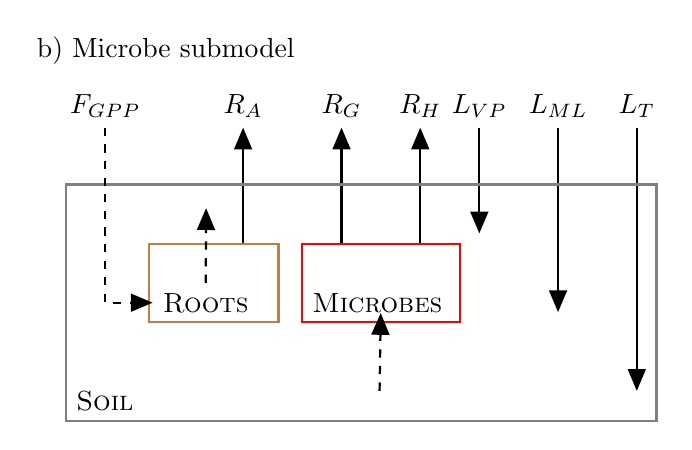
\begin{tikzpicture}[auto, thick, node distance=2cm, >=triangle 45]

\node (A) at (2.5, -0.5) {};
\node (B) at (2.5, 2) {$R_{G}$};

\node (C) at (3.5, -0.5) {};
\node (D) at (3.5, 2) {$R_{H}$};

\node (E) at (1.25, -0.5) {};
\node (F) at (1.25, 2) {$R_{A}$};

\node (G) at (-0.5, 2) {$F_{GPP}$};

\node (Ls) at (4.25, 2) {$L_{VP}$};
\node (Lm) at (5.25, 2) {$L_{ML}$};
\node (Lw) at (6.25, 2) {$L_{T}$};
\node (Ls1) at (4.25, 0.25) {};
\node (Lm1) at (5.25, -0.75) {};
\node (Lw1) at (6.25, -1.75) {};

\node (M) at (3, -0.5) {};
%\node at (0, 2.25) {Microbe \& Microbe-TD};
% arrows
\draw[->] (A) -- (B);
  \draw[->] (C) -- (D);     
  \draw[->] (E) -- (F);

  \draw[->] (Ls) -- (Ls1);     
  \draw[->] (Lw) -- (Lw1);  
    \draw[->] (Lm) -- (Lm1);  
  
  

\node (C1-root) at (-0.4, 0.5)  {};
  
%\draw [dashed,color=gray,thick] (-1.0,0 )-- (8,0);
%\draw [dashed,color=gray,thick] (-1.0,-1 )-- (8,-1);

  
       

	
     	% Boxing and labelling noise shapers
	\draw [color=gray,thick](-1.0,-2) rectangle (6.5,1);  % Overall box
	\draw [color=red,thick,fill=white](2,-0.75) rectangle (4,0.25);  % Microbe box
	\draw [color=brown,thick,fill=white](0.05,-0.75) rectangle (1.7,0.25);  % Root box
	%\draw [color=black,thick,fill=white](4.2,-1.75) rectangle (5.5,.8);  % CA box
	
%	\node (CA) at (4.2,-0.75) [above=2.5mm, right=0mm] {$C_{A}$};
	%\node at (-0.5,1) [above=5mm, right=0mm] {\textsc{Atmosphere}};
	\node (R)  at (0.1,-0.75) [above=2.5mm, right=0mm] {\textsc{Roots}};
	\node (S) at (2.85,-2) [above=2.5mm, right=0mm] {};
	\node  at (2,-0.75) [above=2.5mm, right=0mm] {\textsc{Microbes}};
	\node  at (-1,-2) [above=2.5mm, right=0mm] {\textsc{Soil}};
%	\node (C1) at (6.1, 0.5) {$C_{1}$};
%	\node (C2) at (6.1, -0.5) {$C_{2}$};
%	\node (C3) at (6.1, -1.5) {$C_{3}$};
	
%	\node (CA1) at (4.75, 0.5) {};
%	\node (CA2) at (4.75, -0.5) {};
%	\node (CA3) at (4.75, -1.5) {};	
%	\draw[dashed, ->] (C1) -- (CA1);  
%	\draw[dashed, ->] (C2) -- (CA2);  
%	\draw[dashed, ->] (C3) -- (CA3); 
%	\draw[dashed, ->] (6.5,0.4) -- (6.5,-0.5);   
%	\draw[dashed, ->] (6.8,-0.6) -- (6.8,-1.6);   
%\draw[color=brown, dashed,->] (R) |- (C1-root);
\draw[color=black, dashed,->] (R) -- (0.78,.7);
\draw[color=black, dashed,->] (S) -- (M);
\draw[color=black, dashed,->] (G) |- (R);

\node at (-1.5,2.45) [above=2.5mm, right=0mm] {b) Microbe submodel};


\end{tikzpicture}





%%%%
\vskip 0.5in

%%%  QUALITY MODEL



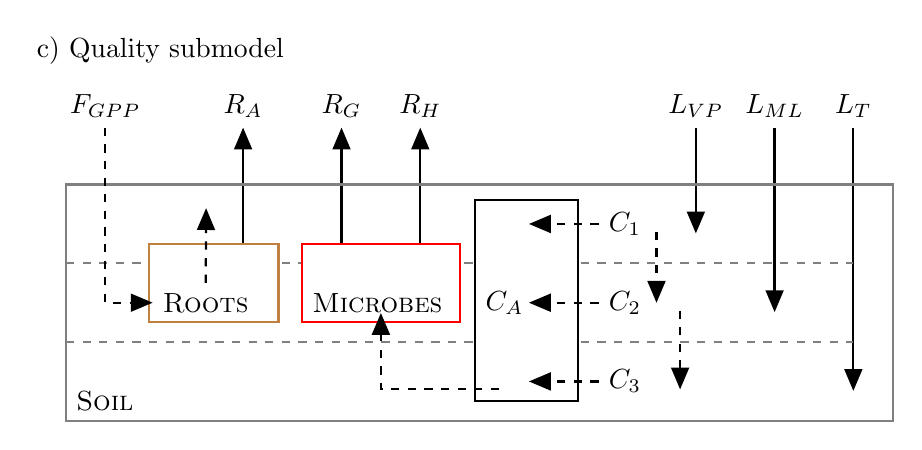
\begin{tikzpicture}[auto, thick, node distance=2cm, >=triangle 45]

\node (A) at (2.5, -0.5) {};
\node (B) at (2.5, 2) {$R_{G}$};

\node (C) at (3.5, -0.5) {};
\node (D) at (3.5, 2) {$R_{H}$};

\node (E) at (1.25, -0.5) {};
\node (F) at (1.25, 2) {$R_{A}$};

\node (G) at (-0.5, 2) {$F_{GPP}$};

\node (Ls) at (7, 2) {$L_{VP}$};
\node (Lm) at (8, 2) {$L_{ML}$};
\node (Lw) at (9, 2) {$L_{T}$};
\node (Ls1) at (7, 0.25) {};
\node (Lm1) at (8, -0.75) {};
\node (Lw1) at (9, -1.75) {};

\node (M) at (3, -0.5) {};
%\node at (0, 2.25) {Microbe \& Microbe-TD};
% arrows
\draw[->] (A) -- (B);
  \draw[->] (C) -- (D);     
  \draw[->] (E) -- (F);

  \draw[->] (Ls) -- (Ls1);     
    \draw[->] (Lm) -- (Lm1);  
  \draw[->] (Lw) -- (Lw1);  
  
  
  

\node (C1-root) at (-0.4, 0.5)  {};
  
\draw [dashed,color=gray,thick] (-1.0,0 )-- (9,0);
\draw [dashed,color=gray,thick] (-1.0,-1 )-- (9,-1);

  
       

	
     	% Boxing and labelling noise shapers
	\draw [color=gray,thick](-1.0,-2) rectangle (9.5,1);  % Overall box
	\draw [color=red,thick,fill=white](2,-0.75) rectangle (4,0.25);  % Microbe box
	\draw [color=brown,thick,fill=white](0.05,-0.75) rectangle (1.7,0.25);  % Root box
	\draw [color=black,thick,fill=white](4.2,-1.75) rectangle (5.5,.8);  % CA box
	
	\node (CA) at (4.2,-0.75) [above=2.5mm, right=0mm] {$C_{A}$};
	%\node at (-0.5,1) [above=5mm, right=0mm] {\textsc{Atmosphere}};
	\node (R)  at (0.1,-0.75) [above=2.5mm, right=0mm] {\textsc{Roots}};
	%\node (S) at (1.5,-2) [above=2.5mm, right=0mm] {\textsc{Soil}};
	\node  at (2,-0.75) [above=2.5mm, right=0mm] {\textsc{Microbes}};
	\node  at (-1,-2) [above=2.5mm, right=0mm] {\textsc{Soil}};
	\node (C1) at (6.1, 0.5) {$C_{1}$};
	\node (C2) at (6.1, -0.5) {$C_{2}$};
	\node (C3) at (6.1, -1.5) {$C_{3}$};
	
	\node (CA1) at (4.75, 0.5) {};
	\node (CA2) at (4.75, -0.5) {};
	\node (CA3) at (4.75, -1.5) {};	
	\draw[dashed, ->] (C1) -- (CA1);  
	\draw[dashed, ->] (C2) -- (CA2);  
	\draw[dashed, ->] (C3) -- (CA3); 
	\draw[dashed, ->] (6.5,0.4) -- (6.5,-0.5);   
	\draw[dashed, ->] (6.8,-0.6) -- (6.8,-1.6);   
%\draw[color=brown, dashed,->] (R) |- (C1-root);
\draw[color=black, dashed,->] (R) -- (0.78,.7);
\draw[color=black, dashed,->] (4.5,-1.6) -| (M);
\draw[color=black, dashed,->] (G) |- (R);

\node at (-1.5,2.45) [above=2.5mm, right=0mm] {c) Quality submodel};


\end{tikzpicture}


%%%%

\end{document}